\documentclass[11pt]{article}

\usepackage[frenchb]{babel}
\usepackage[utf8]{inputenc}
\usepackage[T1]{fontenc}
\usepackage{graphicx}
\usepackage{amsmath}
\usepackage{amsfonts}
\usepackage{stmaryrd}
\usepackage{diagbox}
\usepackage{amsthm}
\usepackage{textcomp}
\usepackage[a4paper,margin=1in]{geometry}
\setcounter{MaxMatrixCols}{20}

\usepackage{float}
\usepackage{empheq}
\usepackage{siunitx}

\usepackage{hyperref}
\usepackage{url}

% \setlength{\voffset}{-0.75in}
% \setlength{\headsep}{5pt}
\usepackage{mathtools}

\title{Rapport du TP d'optimisation et contrôle}
\author{Charles \textsc{Auguste} et Clément \textsc{Riu}}
\date{\today}

\newcommand{\R}{\mathbb{R}^n}

\begin{document}

\maketitle

\section*{Séance 1}

\subsection*{Test de l'oracle avec l'algorithme de gradient à pas fixe}
Afin de tester notre oracle, nous l'avons utilisé avec un algoritmhe de gradient à pas fixe en lançant le programme principal avec la commande\\
\texttt{[fopt,xopt,gopt] = Gradient\_F(OraclePH,xini);}\\
La valeur du pas du gradient est de 0.5, et on réalise 5000 itérations.

\begin{figure}[H]
  \centering
    \includegraphics[width=0.95 \textwidth]{Images/img1.png}
  \caption{Algorithme de descente de gradient à pas fixe.}
\end{figure}

Avec ces données d'entrée, l'algorithme converge. Il faut cependant faire attention car on n'aurait pas forcément convergé pour un pas de gradient trop grand. On voit d'ailleurs que la norme du gradient remonte à un moment. C'est peut être que notre pas de gradient était trop grand à ce moment là. On remarque d'autre part que le pas du gradient est fixe, ce qui est rassurant pour un tel algorithme

\subsection*{Test de l'oracle avec la fonction d'optimisation de Scilab}

On lance le programme principal avec la ligne de commande :\\
\texttt{[fopt,xopt,gopt] = Optim\_Scilab(OraclePGSansCompteur,xini);}\\
On vérifie alors avec les données affichées par le fichier vérification que l'on a bien convergé vers le minimum (les vérifications sont bonnes et la norme du gradient est très proche de 0).


\subsection{Calcul du gradient et du hessien}

On va partir de la relation : $ J(q) = \frac{1}{3}\langle q , r \bullet q \bullet | q | \rangle + \langle pr , A_r q \rangle$ qu'on composera avec $q = q^{(0)} + B q_c$.

\begin{align*}
J(q+h) =& \frac{1}{3}\langle q + h , r \bullet q + h \bullet | q + h | \rangle + \langle pr , A_r (q + h) \rangle \\
=& \frac{1}{3}(\langle q , r \bullet q + h \bullet | q + h | \rangle + \langle h , r \bullet q + h \bullet | q + h | \rangle) + \langle pr , A_r (q + h) \rangle \\
=& \frac{1}{3}(\langle q , r \bullet q \bullet | q + h | \rangle + \langle q , r \bullet h \bullet | q + h | \rangle + \langle h , r \bullet q \bullet | q + h | \rangle + \langle h , r \bullet h \bullet | q + h | \rangle) \\ &+ \langle pr , A_r (q + h) \rangle \\
\text{or : } | q + h | &= |q| + sign(q) h + o(h) \text{ d'où :} \\
=& J(q) + \frac{1}{3}(\langle q , r \bullet q \bullet h sign(q) \rangle + \langle q , r \bullet h \bullet | q | \rangle + \langle h , r \bullet q \bullet | q | \rangle) + \langle pr , A_r h \rangle + o(h) \\
\nabla J(h) =& \langle h , r \bullet q \bullet | q | \rangle) + \langle pr , A_r h \rangle
\end{align*}

D'où le résultat du gradient, \emph{via} $\nabla(q^{(0)} + B q_c) = B$:
$$ \boxed{ \nabla J (q^{(0)} + B q_c) = B^t(r \bullet (q^{(0)} + B q_c) \bullet | q^{(0)} + B q_c | + A_r^t(q^{(0)} + B q_c) } $$

De même le hessien :
$$  \boxed{ H J (q^{(0)} + B q_c) = 2 B^t \text{Diag}(r_i (q^{(0)} + B q_c)_i) B } $$

\subsection*{Équivalence des problèmes}

Soit $q^*$ une solution optimale du problème $(13)$ alors on a $q^* \in U^{ad}_{(14)}$ et la relation $(9)$ montre l'optimalité dans le problème $(14)$ (et comme $U_{(13)}^{ad} \subset U_{(14)}^{ad}$ on a l'équivalence, encore une fois par la relation $(9)$).

\noindent Soit $q^{**}$ solution optimale de $(14)$ en posant $q = q^{(0)} + B q_c$ on a $q^{**}$ solution optimale de $(19)$. Et on a encore l’inclusion des ensemble admissibles, plus la relation $(18)$ qui assure l'équivalence.

\subsection*{Unicité de la solution}

Les critères des problèmes sont continues et s'expriment sous la forme $a q^2|q| + b q$ et donc sont coercifs. La section d'après montre que les problèmes sont strictement convexes.

Par le théorème $(5.3)$ les problèmes admettent une solution et elle est unique.

\subsection*{Convexité}
Soit $x\in \mathbb{R}$ fixé. On pose $h(y) = -x y |x| + \frac{1}{3} y^2 |y| + \frac{2}{3} x^2 |x|$.
 $h'(y) = -x |x| + y^2 sgn(y)$. Donc, $h'(y) = 0 \Leftrightarrow x = y$. Or, la fonction puis croissante, donc la fonction atteint son minimum en x. Or, $h(x) = 0$. Donc pour $y \neq x, h(y) > 0
$. \\

Soit $x\in\R$. On note f la fonction objectif associée au problème 14. La fonction est différentiable donc $\partial f(x) = \{\nabla f(x)\}$.
\begin{align*}
&f(y) - f(x) \\
&= -\frac{1}{3} \langle x,r \bullet x \bullet |x|\rangle  - \langle p_r,A_rx\rangle  + \frac{1}{3}\langle y,r \bullet y \bullet |y|\rangle  + \langle p_r,A_ry\rangle   \\
&= \langle p_r,A_r(y - x)\rangle  + \langle y-x, r \bullet x \bullet |x|\rangle  + \langle r, -y \bullet x \bullet |x| + \frac{1}{3}y \bullet y \bullet |y| + \frac{2}{3}x \bullet x \bullet |x|\rangle \\
&>  \langle y-x,A_t^Tp_r + r \bullet x \bullet |x|\rangle  \tag{les termes que l'on a enlevé étaient positifs par le lemme ci-dessus} \\
&>  D(x;y-x)\\
&\boxed{>  \langle \nabla f(x),y-x\rangle}
\end{align*}

Donc la fonction objectif est strictement convexe par l'exercice 4.60.
D'autre part supposons que $f$ est fortement convexe de module $b$. Soit $\epsilon =  \max_{0\leq i \leq n} \frac{3b}{2nr_i}$. On a pour $x = 0$ et $y = (\epsilon,...,\epsilon)$
\begin{align*}
&f(y) - f(x) \\
&= -\frac{1}{3} \langle x,r \bullet x \bullet |x|\rangle  - \langle p_r,A_rx\rangle  + \frac{1}{3}\langle y,r \bullet y \bullet |y|\rangle  + \langle p_r,A_ry\rangle   \\
&= \langle p_r,A_r(y - x)\rangle  + \langle y-x, r \bullet x \bullet |x|\rangle  + \langle r, -y \bullet x \bullet |x| + \frac{1}{3}y \bullet y \bullet |y| + \frac{2}{3}x \bullet x \bullet |x|\rangle \\
&= \langle A_r^Tp_r,y-x\rangle   + \frac{1}{3}\langle r, \epsilon \bullet \epsilon \bullet \epsilon\rangle  \\
& \boxed{ <  \langle \nabla f(x),y-x\rangle  + \frac{b \epsilon^2}{2} }
\end{align*}
Donc on a une contradiction d'après l'exercice corrigé 4.60. Donc la fonction n'est pas fortement convexe.

Soit $x\in\R$. On note g la fonction objectif associée au problème 19. La fonction est différentiable donc $\partial g(x) = \{\nabla g(x)\}$. On pose $X = q^{(0)} + Bx$ et $Y = q^{(0)} + By$
\begin{align*}
&g(y) - g(x) \\
&= -\frac{1}{3} \langle X,r \bullet X \bullet |X|\rangle  - \langle p_r,A_rX\rangle  + \frac{1}{3}\langle Y,r \bullet Y \bullet |Y|\rangle  + \langle p_r,A_rY\rangle   \\
&= -\frac{1}{3} \langle X,r \bullet X \bullet |X|\rangle  - \langle p_r,A_rBx\rangle  + \frac{1}{3}\langle Y,r \bullet Y \bullet |Y|\rangle  + \langle p_r,A_rBy\rangle   \\
&= \langle B^TA_r^Tp_r,(y - x)\rangle -\frac{1}{3} \langle X,r \bullet X \bullet |X|\rangle + \frac{1}{3}\langle Y,r \bullet Y \bullet |Y|\rangle \\
&= \langle B^TA_r^Tp_r,(y - x)\rangle + \langle B(y-x),r \bullet X \bullet |X|\rangle - \frac{1}{3}\langle q^{(0)},r \bullet X \bullet |X|\rangle + \frac{1}{3}\langle Y,r \bullet Y \bullet |Y|\rangle + \\
&\frac{2}{3} \langle Bx,r \bullet X \bullet |X|\rangle -  \langle By,r \bullet X \bullet |X|\rangle\\
&=  \langle \nabla g(x),y-x\rangle + \frac{1}{3}\langle Y,r \bullet Y \bullet |Y|\rangle + \frac{2}{3} \langle X,r \bullet X \bullet |X|\rangle -  \langle Y,r \bullet X \bullet |X|\rangle \\
& \boxed{ > \langle \nabla g(x),y-x\rangle \tag{Par le lemme du début} }
\end{align*}
Donc la fonction objectif est strictement convexe par l'exercice 4.60. \\
D'autre part supposons que $f$ est fortement convexe de module $b$. Soit $\epsilon>0$. On a pour $x = 0$ et $y = (\epsilon,...,\epsilon)$

\begin{align*}
&g(y) - g(x) \\
&= -\frac{1}{3} \langle X,r \bullet X \bullet |X|\rangle  - \langle p_r,A_rX\rangle  + \frac{1}{3}\langle Y,r \bullet Y \bullet |Y|\rangle  + \langle p_r,A_rY\rangle   \\
&= -\frac{1}{3} \langle X,r \bullet X \bullet |X|\rangle  - \langle p_r,A_rBx\rangle  + \frac{1}{3}\langle Y,r \bullet Y \bullet |Y|\rangle  + \langle p_r,A_rBy\rangle   \\
&= \langle B^TA_r^Tp_r,(y - x)\rangle -\frac{1}{3} \langle X,r \bullet X \bullet |X|\rangle + \frac{1}{3}\langle Y,r \bullet Y \bullet |Y|\rangle \\
&= \langle B^TA_r^Tp_r,(y - x)\rangle + \langle B(y-x),r \bullet X \bullet |X|\rangle - \frac{1}{3}\langle q^{(0)},r \bullet X \bullet |X|\rangle + \frac{1}{3}\langle Y,r \bullet Y \bullet |Y|\rangle + \\
&\frac{2}{3} \langle Bx,r \bullet X \bullet |X|\rangle -  \langle By,r \bullet X \bullet |X|\rangle\\
&=  \langle \nabla g(x),y-x\rangle + \frac{1}{3}\langle Y,r \bullet Y \bullet |Y|\rangle + \frac{2}{3} \langle X,r \bullet X \bullet |X|\rangle -  \langle Y,r \bullet X \bullet |X|\rangle \\
&= \langle \nabla g(x),y-x\rangle + \frac{1}{3}\langle Y,r \bullet Y \bullet |Y|\rangle + \frac{2}{3} \langle q^{(0)},r \bullet q^{(0)} \bullet |q^{(0)}|\rangle -  \langle Y,r \bullet q^{(0)} \bullet |q^{(0)}|\rangle \\
\end{align*}
Puisque les 3 termes de droite tendent vers 0 lorque $\epsilon$ tend vers 0, on voit qu'avec un raisonnement epsilonesque, on montrera le résultat de la même manière que précédemment. On ne détaille pas les calculs car comme mentionné en cours, ce n'est pas l'objet de ce TP.

\section*{Séances 2 et 3}

\subsection*{Autres méthodes}

Pour les méthodes de ces séances, le pas est variable. Voici les courbes que l'on peut obtenir pour ces méthodes. On représente, dans l'ordre, la méthode du gradient de Wolfe, celle de Polakk-Ribière, celle de Newton, et enfin la méthode BFGS.

\begin{figure}[H]
  \centering
    \includegraphics[width=0.95 \textwidth]{Images/gradw.png}
  \caption{Algorithme de descente de gradient à pas variable.}
\end{figure}
\begin{figure}[H]
  \centering
    \includegraphics[width=0.95 \textwidth]{Images/Polak.png}
  \caption{Algorithme de Polak-Ribière.}
\end{figure}
\begin{figure}[H]
  \centering
    \includegraphics[width=0.95 \textwidth]{Images/BGFS.png}
  \caption{Algorithme BFGS.}
\end{figure}
\begin{figure}[H]
  \centering
    \includegraphics[width=0.95 \textwidth]{Images/newton.png}
  \caption{Algorithme de Newton.}
\end{figure}

\subsection*{Comparaison des méthodes}
Pour chaque méthode d'optimisation, on détermine de bons hyperparamètres à la main. Ci-dessous sont listé les résultts pour chaque méthode.
\begin{itemize}
\item Méthode BGFS : pas de 1, convergence en 73 itérations, 376 appels à l'oracle, temps CPU de 0,01 secondes.
\item Méthode Polak-Ribière : pas de 2, convergence en 448 itérations, 3625 appels à l'oracle, temps CPU de 0,80 secondes.
\item Méthode de gradient de Wolfe : pas de 0.01, convergence en 2586 itérations, 36757 appels à l'Oracle, temps CPU de 7,87 secondes (on peut converger en un peu moins d'appels à l'oracle et un peu plus d'itérations avec un pas plus grand, mais l'ordre de grandeur est le même).
\item Méthode de Newton avec recherche linéaire de Wolfe : pas > 1, convergence en 15 itérations, 30 appels à l'oracle, temps CPU de 0.03 secondes.
\item Méthode du gradient à pas fixe : Pas de 1, plus de 5000 itérations (le gradient ne converge pas même si on a bien le bon critère optimal), plus de 5000 appels à l'oracle, temps CPU de 2,11 secondes.
\end{itemize}

Toutes les méthodes convergent vers le même critère optimal : 3,734 environ.
Nos temps CPU sont cohérents avec ceux de la fonction d'optimisation de Scilab : ce sont les mêmes.
La méthode BFGS est la plus rapide suivie de la méthode de Newton, puis de la méthode de Polak-ribière. Cependant, si les appels à l'oracle étaient très couteux, on pourrait avoir recours à la méthode de Newton car elle demande beaucoup moins d'appels à l'oracle, même si elle nécessite d'inverser une hessienne.
Les méthodes avec les gradients à pas fixes ou conjugués demandent beaucoup d'appels à l'oracle, ce qui pourrait être embêtant si l'oracle était plus complexe à calculer.


\section*{Séance 4}

\paragraph{1.} ~\\


Si on appelle $\lambda$ le vecteur des coefficients de Lagrange, on a le lagragien :

\begin{align*}
  \boxed{ \mathcal{L}(q, \lambda) = \frac{1}{3} \langle q, r \bullet q \bullet |q| \rangle + \langle p_r, A_r q \rangle + \langle \lambda , A_d q - f_d \rangle }
\end{align*}

Les conditions d'optimalités (théorème $6.8$ du cours) nous font étudier les points selles du lagrangien pour trouver l'optimum, nous allons donc étudier :

\begin{align*}
  \left\{
  \begin{array}{lcl}
    \nabla_q \mathcal{L}(q , \lambda) & = & 0 \\
    \nabla_{\lambda} \mathcal{L}(q, \lambda) & = & 0
  \end{array}
  \right.
\end{align*}

Utilisons les résultats des calculs des questions suivantes pour étudier le lagrangien :

\begin{align*}
  &\left\{
  \begin{array}{lcl}
    \nabla_q \mathcal{L}(q , \lambda) & = & r \bullet q \bullet |q| + A_r^t p_r + A_d^t \lambda \\
    \nabla_{\lambda} \mathcal{L}(q, \lambda) & = & A_d q - f_d
  \end{array}
  \right.
  \\
  &\left\{
  \begin{array}{lcl}
    0 & = & r \bullet q \bullet |q| + A_r^t p_r + A_d^t \lambda \\
    0 & = & A_d q - f_d
  \end{array}
  \right.
  \\
  &\left\{
  \begin{array}{lcl}
    0 & = & r \bullet q \bullet |q| + A^t \begin{pmatrix} p_r \\ \lambda \end{pmatrix} \\
    0 & = & A_d q - f_d
  \end{array}
  \right.
\end{align*}

On retrouve bien, sur les données du problèmes, les relations $(6)$ et $(8)$. On peut aussi en déduire que $\lambda$ représente les préssions aux n\oe{}uds réservoirs.

\paragraph{2.} ~\\


On cherche le maximiseur $\hat{q}$ en fonction de $\lambda$, soit un point où le gradient en $q$ du lagrangien s'annule :

\begin{align*}
  \mathcal{L}(q + h, \lambda) = \frac{1}{3} \langle q + h, r \bullet q + h \bullet |q + h| \rangle + \langle p_r, A_r (q + h) \rangle + \langle \lambda , A_d (q + h) - f_d \rangle
\end{align*}

Donne, grâce au résultat de la partie 1 :

\begin{align*}
  \nabla_q \mathcal{L}(q, \lambda) = r \bullet q \bullet |q| + A_r^t p_r + A_d^t \lambda
\end{align*}

On peut donc écrire :

\begin{align*}
  \nabla_q \mathcal{L}(\hat{q} , \lambda) &= 0 \\
  r \bullet \hat{q} \bullet |\hat{q}| + A_r^t p_r + A_d^t \lambda &= 0
\end{align*}

Soit, en posant $z = A_r^t p_r + A_d^t \lambda$ et en écrivant $a^{-1 \bullet} \coloneqq \begin{bmatrix} \frac{1}{a_i} \end{bmatrix}_i$ si $\forall i, b_i \ne 0$ et en notant : $\sqrt[\bullet]{a} = \begin{bmatrix} \sqrt{a_i} \end{bmatrix}_i$ si $\forall i, a_i \ge 0$ :

\begin{align*}
  r \bullet \hat{q} \bullet |\hat{q}| &= - z \\
  \hat{q} \bullet |\hat{q}| &= -z \bullet r^{-1 \bullet} \\
  \hat{q} &= \boxed{ - \sqrt[\bullet]{|z \bullet r^{-1 \bullet}|} \bullet \text{sign}(z \bullet r^{-1 \bullet}) }
\end{align*}

À partir de là, on peut écrire le lagrangien avec seulement une dépendance en $\lambda$ :

\begin{align*}
  \mathcal{L}(\lambda) =& \frac{1}{3} \langle - \sqrt[\bullet]{|z \bullet r^{-1 \bullet}|} \bullet \text{sign}(z \bullet r^{-1 \bullet}), r \bullet - \sqrt[\bullet]{|z \bullet r^{-1 \bullet}|} \bullet \text{sign}(z \bullet r^{-1 \bullet}) \bullet |- \sqrt[\bullet]{|z \bullet r^{-1 \bullet}|} \bullet \text{sign}(z \bullet r^{-1 \bullet})| \rangle \\
  &+ \langle p_r, A_r - \sqrt[\bullet]{|z \bullet r^{-1 \bullet}|} \bullet \text{sign}(z \bullet r^{-1 \bullet}) \rangle \\
  &+ \langle \lambda , A_d - \sqrt[\bullet]{|z \bullet r^{-1 \bullet}|} \bullet \text{sign}(z \bullet r^{-1 \bullet}) - f_d \rangle
\end{align*}

À partir de ce résultat nous obtenons facilement le gradient et le hessien en $\lambda$ du lagrangien à l'optimum :

\begin{align*}
   \nabla_{\lambda} \mathcal{L}(\lambda) &= \boxed{ A_d (- \sqrt[\bullet]{|z \bullet r^{-1 \bullet}|} \bullet \text{sign}(z \bullet r^{-1 \bullet})) - f_d } \\
   H_{\lambda} \mathcal{L}(\lambda) &= \boxed{ \frac{1}{2} A_d \text{diag}\Bigg(\bigg(- \text{sign}(z \bullet r^{-1 \bullet}) \bullet \sqrt[\bullet]{|z \bullet r^{-1 \bullet}|}^{-1 \bullet}\bigg) \bullet \bigg( \text{sign}(z) \bullet \sqrt[\bullet]{|z|}^{-1 \bullet}\bigg)\Bigg) A_d^t }
\end{align*}

\paragraph{3.} Voir fichier \texttt{Oracle\_lagrange.sci}.

\paragraph{4.} ~\\

Lorsqu'on appelle l'oracle implémentant le problème dual, on obtient des résultats bons (le code de vérification renvoie des erreurs quasi nulles). Ces résultats confirment la théorie : le problème dual donne la même solution que le problème primal.

Traçons les différentes évolutions en fonction des algorithmes (voir plus bas).
Dans un premier temps, on remarque que l'algorithme de descente de gradient à pas fixe et l'algorithme de descente de gradient à pas variable arrive au maximum d'itérations autorisées avant d'avoir atteint le seuil de précision défini. L'algorithme du gradient à pas variable a donc moins bien convergé pour le dual que pour le primal.

Néanmoins, pour comparer les différents algorithmes entre eux l'oracle que l'algorithme de Newton est le plus rapide ($0,052s$), suivi de BFGS ($0,22s$) puis l'algorithme de Polak-Ribière ($1,408s$) est un peu plus lent. Nous ne notterons pas les résultats des algorithmes de descente de gradient, car ceux-ci n'ont pas convergés.

\begin{figure}[H]
  \centering
    \includegraphics[width=0.95 \textwidth]{Images/Lagrange_pas_fixe.eps}
  \caption{Algorithme de descente de gradient à pas fixe. En haut, en rouge l'évolution de la norme du gradient en fonction des itérations ou des appels à l'oracle. En bleu, l'évolution du pas en fonction des itérations.}
\end{figure}

\begin{figure}[H]
  \centering
    \includegraphics[width=0.95 \textwidth]{Images/Lagrange_pas_vari.eps}
  \caption{Algorithme de descente de gradient à pas variable. En haut, en rouge l'évolution de la norme du gradient en fonction des itérations ou des appels à l'oracle. En bleu, l'évolution du pas en fonction des itérations.}
\end{figure}

\begin{figure}[H]
  \centering
    \includegraphics[width=0.95 \textwidth]{Images/Lagrange_pol_ribi.eps}
  \caption{Algorithme de Polak-Ribière. En haut, en rouge l'évolution de la norme du gradient en fonction des itérations ou des appels à l'oracle. En bleu, l'évolution du pas en fonction des itérations.}
\end{figure}

\begin{figure}[H]
  \centering
    \includegraphics[width=0.95 \textwidth]{Images/Lagrange_alg_BFGS.eps}
  \caption{Algorithme BFGS. En haut, en rouge l'évolution de la norme du gradient en fonction des itérations ou des appels à l'oracle. En bleu, l'évolution du pas en fonction des itérations.}
\end{figure}

\begin{figure}[H]
  \centering
    \includegraphics[width=0.95 \textwidth]{Images/Lagrange_alg_Newt.eps}
  \caption{Algorithme de Newton. En haut, en rouge l'évolution de la norme du gradient en fonction des itérations ou des appels à l'oracle. En bleu, l'évolution du pas en fonction des itérations.}
\end{figure}

\end{document}
